\documentclass[11pt,letterpaper,english]{article}

% Page design
\usepackage[top=1in, bottom=1in, left=1in, right=1in] {geometry}
\pagestyle{empty}

% General packages
\usepackage[T1]{fontenc}
%\usepackage{txfonts}
\usepackage{xcolor}
%\usepackage{eqnarray}
\usepackage{epsfig}
\usepackage{epstopdf}
\usepackage{graphicx}
\usepackage{mathptmx}
\usepackage{enumitem}
\usepackage{booktabs}
\usepackage{setspace}
\newcommand{\verbatimfont}[1]{\renewcommand{\verbatim@font}{\ttfamily#1}}
\usepackage{graphicx}
\usepackage{epstopdf}
\usepackage{color}
\usepackage{multirow}
\usepackage{floatrow}
\usepackage{bm}
\usepackage{amsmath}
\usepackage{hhline}
\setlength\doublerulesep{.7pt}
%\usepackage{tabularx}
\usepackage{subcaption}

%\usepackage{csmacros}
\usepackage{dsfont}
%%-------------------------------------------------------------------------------

% This file is part of Code_Saturne, a general-purpose CFD tool.
%
% Copyright (C) 1998-2018 EDF S.A.
%
% This program is free software; you can redistribute it and/or modify it under
% the terms of the GNU General Public License as published by the Free Software
% Foundation; either version 2 of the License, or (at your option) any later
% version.
%
% This program is distributed in the hope that it will be useful, but WITHOUT
% ANY WARRANTY; without even the implied warranty of MERCHANTABILITY or FITNESS
% FOR A PARTICULAR PURPOSE.  See the GNU General Public License for more
% details.
%
% You should have received a copy of the GNU General Public License along with
% this program; if not, write to the Free Software Foundation, Inc., 51 Franklin
% Street, Fifth Floor, Boston, MA 02110-1301, USA.

%-------------------------------------------------------------------------------

\newcommand{\CS}{%
  {\fontfamily{ppl}\fontshape{it}\selectfont Code\_Saturne}\xspace}
\newcommand{\verscs}{5.3-alpha\xspace}
\newcommand{\revscs}{bd6ad94-m\xspace}


% Section format
\usepackage{sectsty}
\sectionfont{\normalsize}
\subsectionfont{\normalsize}
\subsubsectionfont{\normalsize \it}
\usepackage{titlesec}
\setlength{\parskip}{\baselineskip}
\setlength{\parindent}{0pt}

\titlespacing\section{0pt}{0\parskip}{0\parskip}
\titlespacing\subsection{0pt}{0\parskip}{0\parskip}
\titlespacing\subsubsection{0pt}{0\parskip}{0\parskip}
\titleformat{\section}[block]{\normalfont\normalsize\bfseries}{\thesection .}{1em}{}
\titleformat{\subsection}[block]{\normalfont\normalsize\bfseries}{\thesubsection .}{1em}{}
\titleformat{\subsubsection}[block]{\normalfont\normalsize\bfseries}{\thesubsubsection .}{1em}{}


% Bibliography format

\usepackage[hidelinks]{hyperref}
\usepackage[numbers]{natbib}
\usepackage{doi}
\renewcommand{\refname}{REFERENCES}
\makeatletter
\renewcommand\@biblabel[1]{#1.\em}
\makeatother
\setlength{\bibsep}{0pt plus 0.3ex}

% Captions
\usepackage{caption}
\captionsetup[figure]{labelfont={bf,normalsize},textfont={bf,normalsize},labelformat={default},labelsep=period,name={Figure}}

% Tables
\floatsetup[table]{capposition=top}
\captionsetup[table]{labelfont={bf,normalsize},textfont={bf,normalsize},labelformat={default},labelsep=period,name={Table}}
\renewcommand{\thetable}{\Roman{table}}
\captionsetup[sub]{font={normalsize},labelfont={bf,normalsize}}

% UDF
\definecolor{brown}{RGB}{74,68,42}
\newcommand{\tw}[1]{#1\textwidth}
\newcommand{\lw}{\linewidth}
\renewcommand{\eqref}[1]{(\ref{#1})}

\raggedright

\begin{document}
\vspace*{-0.45in}
\begin{center}
{\Large\centering\bf TOWARD THE DIRECT NUMERICAL SIMULATION OF A 5X5 ROD BUNDLE }

\vspace{3pt}

{\bf \large Elia Merzari, Thomas Noordine and Oana Marin} \\
\large Argonne National Laboratory \\
\large 9700 S. Cass Avenue, Lemont IL 60439, USA \\
{\color{brown} emerzari@anl.gov,  tnorddine@anl.gov, oanam@mcs.anl.gov}

\vspace{3pt}

{\bf \large Sofiane Benahmadouche} \\
\large  Electricite de France \\
\large 78401 Chatou Cedex, France \\
{\color{brown}  sofiane.benhamadouche@edf.fr}

\end{center}



\normalsize

\section*{ABSTRACT}

Rod bundle flows are prevalent in nuclear engineering for both light water reactors (LWR) and advanced reactor concepts. Unlike canonical channel flow the flow in rod bundles presents some unique characteristic that have evaluate over decades of  experimental and numerical research. Among the most interesting characteristics of rod bundles versus canonical flows is certainly the inhomogeneous cross section which can present different local conditions of turbulence as well as the presence of localized effects characteristics of external flows.
Despite the widespread presence of rod-bundle flows and the decades of knowledge acquired in this field, there are no publicly available direct numerical simulations (DNS) of the flow in multiple-pin rod bundles with heat transfer. In fact, there is only little data available for single-pin infinite-lattice bundles, which are of limited in practical applications as wall effects in the cross section are always important. A multiple-pin DNS study is of great value to the engineering community  as it would allow for the assessment of the reliability of various turbulence models in the presence of heat transfer. Moreover such simulation would provide an invaluable source of data for a deeper understanding of the flow physics.
In this work we present work toward the direct numerical simulation of the flow in a 5 by 5 rod bundle representative of LWR fuel. We consider standard configurations as well as configurations where the central pin is removed and replaced with a guide thimble. The thimble is larger in diameter than the pin and contributed to adding greatly to the non-uniformity of the flow in the cross section. We perform simulations in Code\_Saturne to design the numerical DNS experiment to be performed ith the open source spectral element code Nek5000. Large Eddy Simulations are also performed in Nek5000 to confirm that the resolution requirements are adequate,   We also analyze the anisotropy of the Reynolds stress tensor and compare results from Code\_Saturne and Nek5000.

\begin{flushright}
{\bf KEYWORDS} \\
Rod bundle, LES, DNS, Nek5000
\end{flushright}

\section{INTRODUCTION}

Rod bundles are an essential component of most nuclear reactors concepts. Th external flow over arrays of cylindrical rods is therefore of great interest to nuclear engineers and reactor designers. The prediction of the temperature distribution within the rod bundle is of particular importance. Unlike in canonical channel flow, the flow in rod bundles presents some unique characteristic that have evaluate over decades of  experimental and numerical research. Among the most interesting characteristics of rod bundles versus canonical flows is certainly the inhomogeneous cross section which can present different local conditions of turbulence as well as the presence of localized effects characteristics of external flows.
Historically, System codes and subchannel codes have been extensively used in the thermal-hydraulic analysis of reactor fuel assemblies, but they are limited by the need of empirical correlations derived from representative experimental results over a range of parameters.
Computational Fluid Dynamics (CFD) has emerged in the last two decades as a promising solution to predict flow and heat transfer in rod bundles.
Industry relies routinely on Reynolds Averaged Navier-Stokes (RANS) approaches to predict the flow in rod bundles with LWR spacer grids. The simulation of wire-wrapped rod bundles has also been an active topic of research. RANS retains some limitations due to the need to provide closure relationships and beenfit from comparison with turbulence resolving techniques.Such High fidelity techniques, including direct numerical simulations (DNS) or highly resolved large eddy simulations (LES), allow for an accurate computation of the flow and heat transfer phenomena in nuclear assemblies, without the need of empirical correlations. Their cost however scales with the Reynolds number and remain prohibitive for realistic geometries.
We note that despite the wealth of literature available on rod bundles, there are no publicly available direct numerical simulations (DNS) of the flow in multiple-pin rod bundles with heat transfer. In fact, there is only little data available for single-pin infinite-lattice bundles, which are of limited in practical applications as wall effects in the cross section are always important. A multiple-pin DNS study is of great value to the engineering community  as it would allow for the assessment of the reliability of various turbulence models in the presence of heat transfer. Moreover such simulation would provide an invaluable source of data for a deeper understanding of the flow physics.
In this work we present work toward the direct numerical simulation of the flow in a 5 by 5 rod bundle representative of LWR fuel. We consider standard configurations as well as configurations where the central pin is removed and replaced with a guide thimble. The thimble is larger in diameter than the pin and contributed to adding greatly to the non-uniformity of the flow in the cross section. We perform simulations in Code\_Saturne to design the numerical DNS experiment to be performed with the open source spectral element code Nek5000. Large Eddy Simulations are also performed in Nek5000 to confirm that the resolution requirements are adequate,   We also analyze the anisotropy of the Reynolds stress tensor and compare results from Code\_Saturne and Nek5000.
The numerical methods are summarized in Section~\ref{methods}. The results from Code\_Saturne used for the design of the numerical experiment are summarized in Section~\ref{results_saturne} while numerical results for Nek5000 are summarized in Section~\ref{results_nek5000}. Finally a discussion is provided in Section~\ref{discussion}.

\section{METHODS}
\label{methods}

Let us consider the velocity (Eq. \eqref{UEqn}), continuity (Eq. \eqref{rhoEqn}) and energy (Eq. \eqref{EEqn}) equations, that describe incompressible flow of a Newtonian fluid in the absence of other body or external forces.
\begin{equation}
\frac{\partial  u_i  }{\partial t} +  \frac{\partial}{\partial x_j} \left( u_i u_j \right) =-\frac{1}{\rho} \frac{\partial p}{\partial x_i} + \frac{\partial}{\partial x_j} \left[ \nu \left( \frac{\partial u_i}{\partial x_j} +\frac{\partial u_j}{\partial x_i} \right) \right]
\label{UEqn}
\end{equation}
\begin{equation}
\frac{\partial u_i}{\partial x_i} = 0
\label{rhoEqn}
\end{equation}
\begin{equation}
\rho c_p \left( \frac{\partial T }{\partial t} + u_j \frac{\partial T}{\partial x_j} \right) = \frac{\partial }{\partial x_j} \left( \lambda \frac{\partial T}{\partial x_j} \right)
\label{EEqn}
\end{equation}
where $\rho$ is the constant density of the fluid, $\nu$ represents the kinematic viscosity, $\lambda$ is the thermal conductivity and $c_p$ the heat capacity. Implicit summation applies. Let us also note here, that if the fluid viscosity does not depend on temperature (a valid assumption for the cases that are considered for the proposed methodology), velocity equations are completely uncoupled to the temperature field. For the sake of simplicity, thermal conductivity and the heat capacity will also be considered constant. Using the Reynolds averaging operator, one may divide instantaneous fields in an average part (time average for statistically steady flows) and a fluctuating part (i.e. $u_i = \overline{u}_i+u_i'$). When this is applied to NS equations, the RANS equations are obtained (Eqs. \eqref{UEqnRANS}, \eqref{rhoEqnRANS} and \eqref{EEqnRANS}).
\begin{equation}
\frac{\partial  \overline{u}_i  }{\partial t} +  \frac{\partial}{\partial x_j} \left( \overline{u}_i \overline{u}_j \right) =-\frac{1}{\rho} \frac{\partial \overline{p}}{\partial x_i} + \frac{\partial}{\partial x_j} \left[ \nu \left( \frac{\partial \overline{u}_i}{\partial x_j} +\frac{\partial \overline{u}_j}{\partial x_i} \right) \right] + \frac{\partial}{\partial x_j }\left( -\overline{u_i' u_j'} \right)
\label{UEqnRANS}
\end{equation}
\begin{equation}
\frac{\partial \overline{u}_i}{\partial x_i} = 0
\label{rhoEqnRANS}
\end{equation}
\begin{equation}
 \frac{\partial \overline{T} }{\partial t} + \overline{u}_j \frac{\partial \overline{T}}{\partial x_j}  = \frac{\partial }{\partial x_j} \left( \alpha \frac{\partial \overline{T}}{\partial x_j} \right) +\frac{\partial}{\partial x_j} \left( -\overline{u_j' T'}\right)
\label{EEqnRANS}
\end{equation}
where constant density and heat capacity have been absorbed in the thermal diffusivity ($\alpha = \lambda / (\rho c_p)$). The additional terms that appear in velocity and energy equations represent respectively the Reynolds stress tensor ($-\overline{u_i' u_j'} $) and the turbulent heat fluxes ($ -\overline{u_j' T'}$). Different closures for those terms lead to the variety of RANS and turbulent heat fluxes models available in literature.

\subsection{Code\_Saturne}

Pseudo 2D calculation have been performed with the open source finite volume code Code\_Saturne to estimate the Taylor microscale ( $ \lambda = \sqrt{\frac{15 k \nu}{\epsilon}} $) and the Kolmogorov scale( $ \eta = (\frac{\nu^{3}}{\epsilon})^{\frac{1}{4}}$). The results have been used to design the LES and DNS numerical experiments performed with Nek5000. The mesh DNS mesh has been designed so that the distance between GLL points is smaller than min($\frac{\lambda}{2}$,$\eta$).

An Elliptic Blending Reynold's Stress Model\cite{manceau2002} has been used, the following set of coupled equations has been solved : 

%\begin{equation}
%  \frac{\partial R_{ij}}{\partial t} + u_{k}\frac{\partial R_{ij}}{\partial x_{k}} = d_{ij} + P_{ij} + G_{ij} + \Phi_{ij} - \epsilon_{ij}
%\end{equation}

\begin{equation}
\begin{split}
  \frac{\partial R_{ij}}{\partial t} + u_{k}\frac{\partial R_{ij}}{\partial x_{k}} = & -\rho ( R_{ij}S_{ji} + R_{ij}S_{ij} ) - C_{s} \frac{\partial}{\partial x_{k}}( \rho\frac{k}{\epsilon} R_{km}\frac{\partial R_{ij}}{\partial x_{m}}) \\ 
  & + (1-\alpha^{3})(\Phi_{ij}^{w} -\epsilon_{ij}^{w}) + \alpha^{3}(\Phi_{ij}^{h} - \epsilon_{ij}^{h})
\end{split}
\end{equation}

The main idea of the EBRSM, based on the Durbin's blending approach, is to get the correct wall assymptotic behavior for the pressure correlation term $\underline{\underline{\Phi}}$ and represent the blocking of the wall normal fluctuations.
The elliptic blending functions $f_{\Phi}$ and $f_{\epsilon}$\cite{manceau2015} have been set equal to $\alpha^{3}$, which are the default values in Code\_Saturne.


%\begin{equation}
%  p_{ij} = -\rho ( R_{ij}S{ji} + R_{ij}S{ij} )
%\end{equation}
%\begin{equation}
%  d_{ij} = - C_{s} \frac{\partial}{\partial x_{k}}( \rho\frac{k}{\epsilon} R_{km}\frac{\partial R_{ij}}{\partial x_{m}})
%\end{equation}
%\begin{equation}
%  \epsilon_{ij} = (1-Ak\alpha)\epsilon_{ij}^{w} + Ak\alpha*\epsilon_{ij}^{h}
%\end{equation}
%\begin{equation}
%  \underline{\underline{\Phi}} = (1-Ak\alpha)\underline{\underline{\Phi}}^{w} + Ak\alpha*\underline{\underline{\Phi}}^{h}
%  \Phi_{ij} = (1-Ak\alpha)\Phi_{ij}^{w} + Ak\alpha*\Phi_{ij}^{h}
%\end{equation}

\begin{equation}
%  \underline{\underline{\epsilon}}^{w} = \frac{\overline{\underline{\underline{R}}}}{k}\epsilon \text{ and } \underline{\underline{\epsilon}}^{h} = \frac{2}{3} \epsilon \underline{\underline{\mathds{1}}}
  \epsilon_{ij}^{w} = \frac{\overline{R}_{ij}}{k}\epsilon \text{ and } \epsilon_{ij}^{h} =\frac{2}{3} \epsilon \delta_{ij}
\end{equation}

\begin{equation}
%  \underline{\underline{\epsilon}}^{w} = \frac{\overline{\underline{\underline{R}}}}{k}\epsilon \text{ and } \underline{\underline{\epsilon}}^{h} = \frac{2}{3} \epsilon \underline{\underline{\mathds{1}}}
  \Phi_{ij}^{w} = -5.0 \frac{\epsilon}{k} (R_{ik}n_{j}n_{k} + R_{jk} n_{i} n_{k} - \frac{1}{2} (R_{kl}n_{k}n_{l}n_{i}n_{j}-R_{kl}n_{k}n_{l}\delta_{ij})) 
\end{equation}
\begin{equation}
%  \Phi_{ij}^{h} = -C_{1}\frac{\epsilon}{k}(R_{ij}-\frac{2}{3}k\delta_{ij}) - C_{2}(P_{ij} - \frac{2}{3}P_{kk}\delta_{ij}) 
  \Phi_{ij}^{h} = -C_{1}\epsilon a_{ij} -C_{2}P_{k}a_{ij} + (C_{3} - C_{3}'\sqrt{a_{kl}a_{kl}})k S_{ij} + C_{4}k(a_{ik}S_{jk} + a_{jk}S_{ik} - \frac{2}{3} a_{kl} S_{kl} \delta_{ij}) + C_{5}k(a_{ik}W_{jk} + a_{jk}W_{ik})%+ C_{1}\epsilon(a_{ik}a_{kj}- \frac{1}{3}A_{2}\delta_{ij})
\end{equation}

The elliptic blending factor,$\alpha$ is solution of the following elliptic equation :
\begin{equation}
  \alpha - L^{2} \nabla^{2} \alpha = \frac{1}{k} 
\end{equation}
and $n_{i} = \frac{(\nabla \alpha)_{i}}{||(\underline{\nabla} \alpha)||}$, the unit normal of the $\alpha$ gradient

This the EBRSM is a near wall model, $y^{+} = 0.5$ and $x^{+} = 3.5$ have consequently been targeted and checked a posteriori. A 3D mesh composed of hexahedral elements has been created with the mesh generator Gmsh and extruded over a single layer. Periodicity conditions has been et in the steam-wise direction and a local pressure gradient used to ensure a constant bulk velocity during the simulation. The physical quantities have been averaged after convergence to get rid of potential numerical fluctuations.
A space centered scheme and a second order time stepper has been used. the set of 6 $R_{ij}$ equations have been solved with the coupled solver in Code\_Saturne.

\begin{figure}
  \begin{center}
    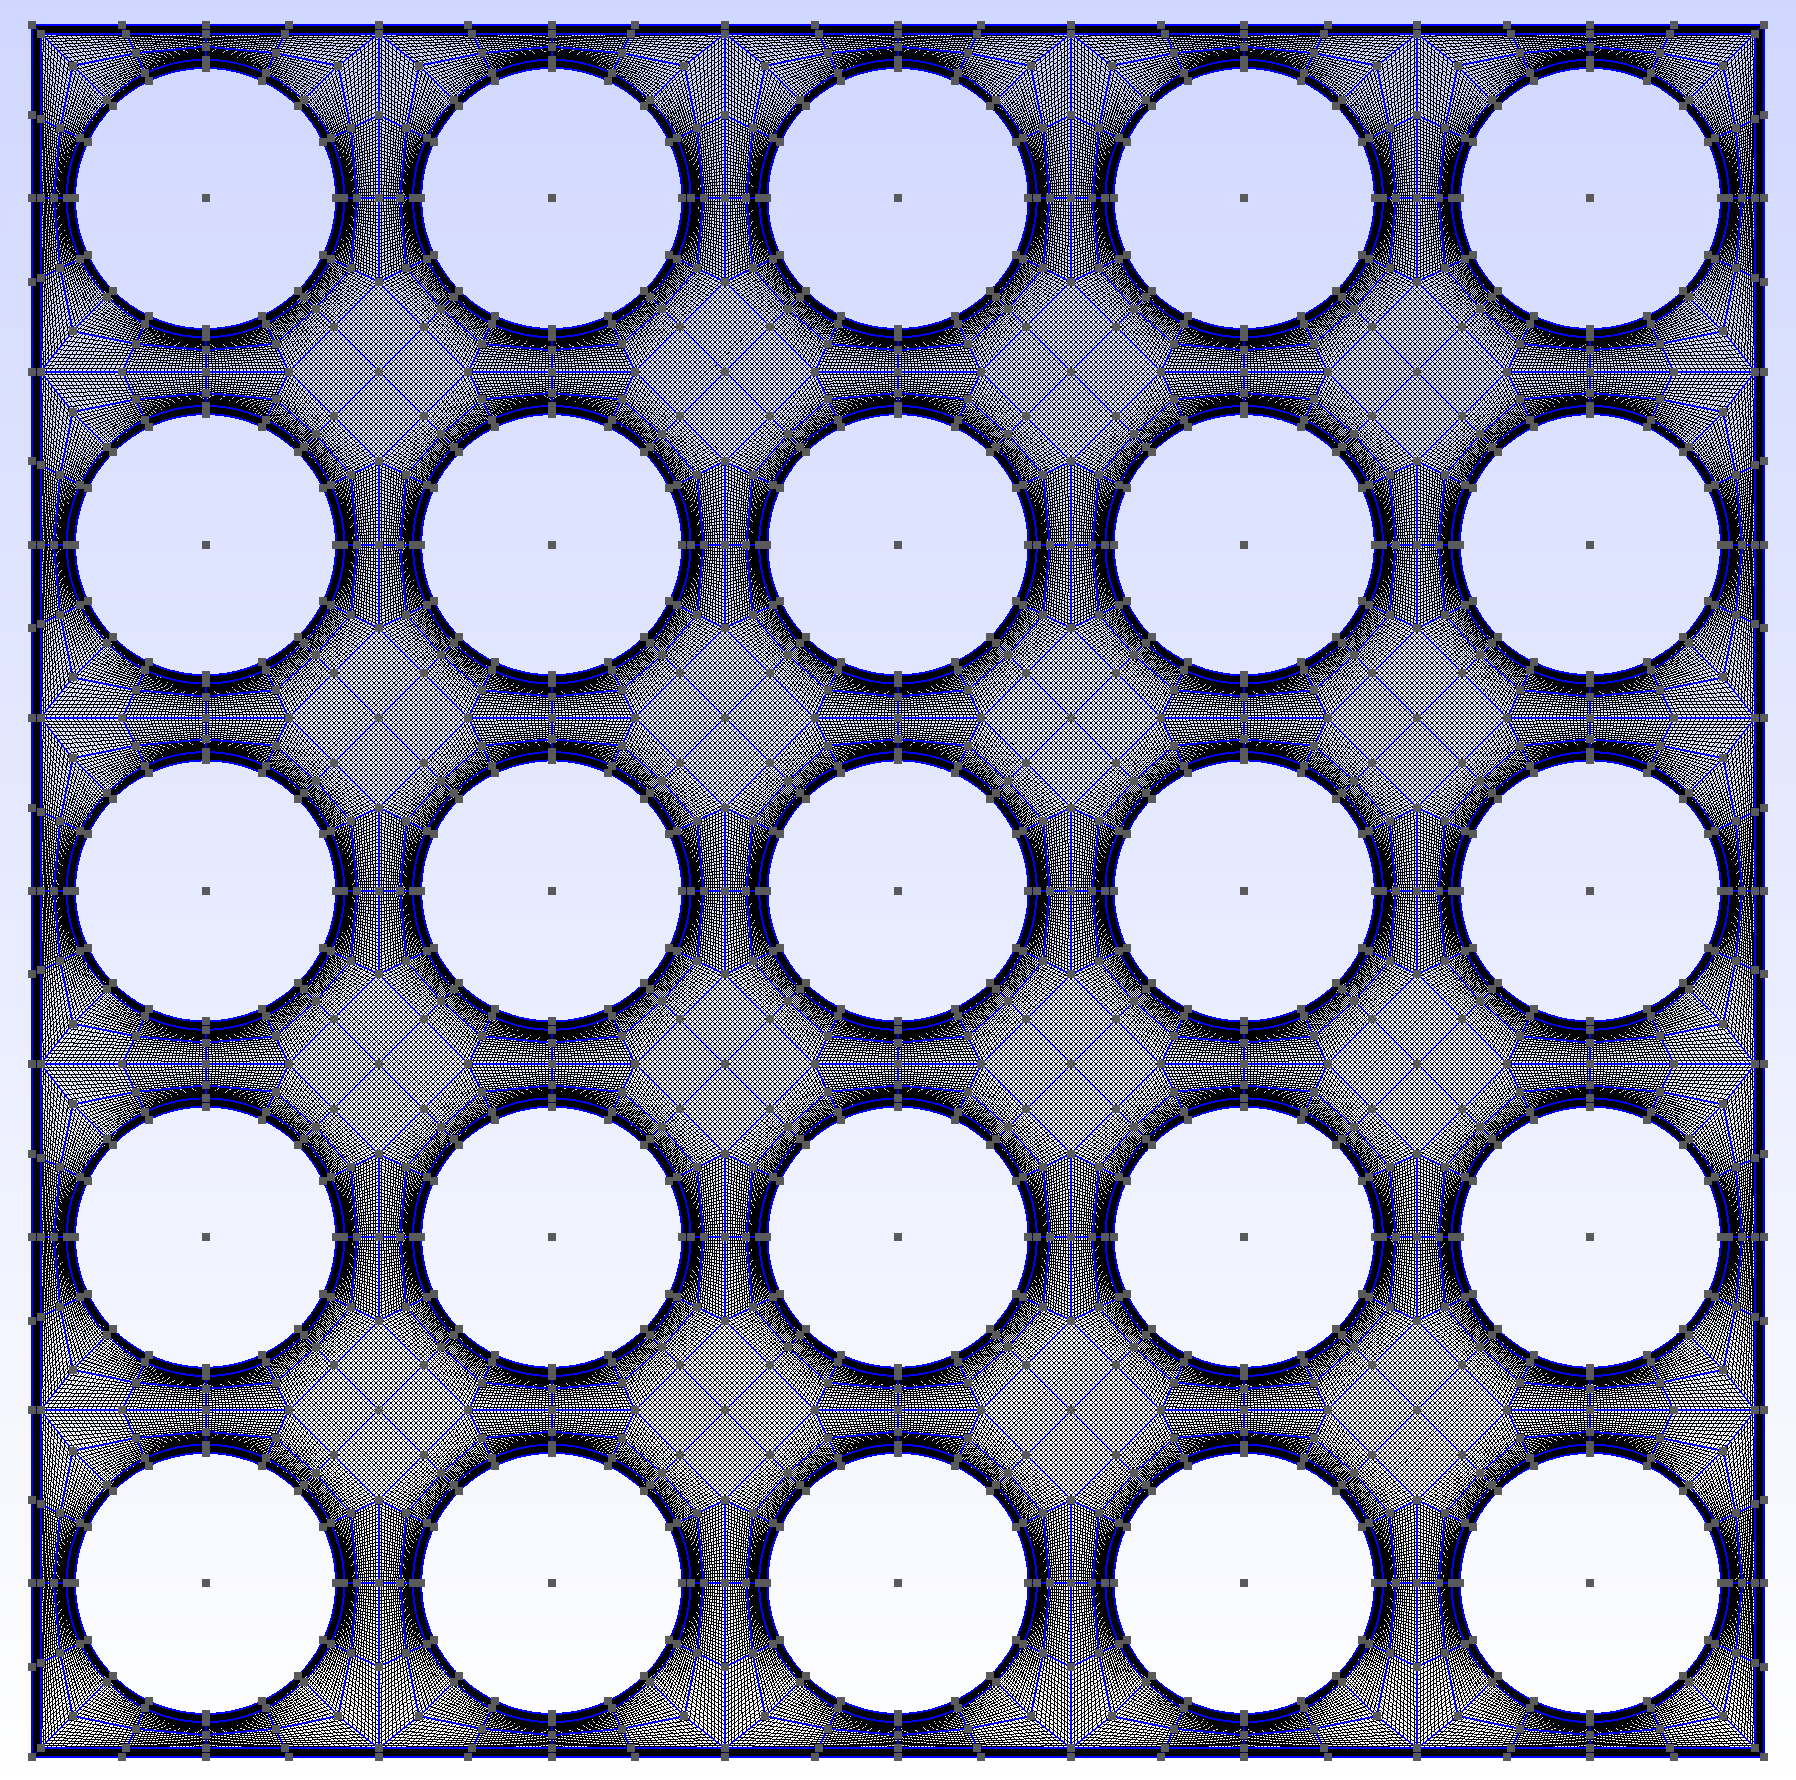
\includegraphics[height = 50mm]{./Figures/ss_thimble/ss_thimble_mesh.png}
    \caption{2D periodic mesh used with Code\_Saturne.}
  \end{center}
\end{figure}





\subsection{Nek5000}
The LES simulations have been performed with the high-order spectral element code Nek5000 \cite{fischer2002}. the planned DNS calculations will also be performed with Nek5000. The Spectral Element Method (SEM), introduced by Patera \cite{patera1984} is a subclass of the Galerkin methods. SEM combines the geometric flexibility of finite elements with the minimal numerical dispersion and dissipation of spectral methods, making it well suited for DNS and highly resolved LES computations of simple to complex geometries. The domain is discretized into $E$ curvilinear hexahedral elements, in which the solution is represented as a tensor-product of $N^{th}$-order Lagrange polynomials based on the Gauss-Lobatto-Legendre (GLL) nodal points, leading to a total of $n\approx E (N+1)^3$ degrees or freedom per scalar field. Nek5000 was designed from the outset for distributed-memory platforms. It is highly parallel and has been recently applied to a variety of problems to gain unprecedented insight into the physics of turbulence in complex flows \cite{obabko2015}. Time-stepping is semi-implicit: the viscous terms of the NS equations are treated implicitly (for the current simulations a second-order backward differentiation has been used,  BDF2), while non-linear terms are treated by a third order extrapolation (EXT3) scheme. The main bottleneck of these computations is the resolution of the elliptic problem for the governing pressure. The discrete Poisson equation is solved using a variational multigrid GMRES method with $local$ overlapping Schwarz methods for element-based smoothing at resolution $N$ and $\approx N/2$, coupled with a $global$ coarse-grid problem based on linear elements \cite{fischer2005}. The LES formulation relies on explicit filtering \cite{slotz2005} of modes $k=N-1$ and $k=N$, which provides an energy drain at the unresolved grid scale, similar to deconvolution LES models. For the presented LES simulations 1\% filtering of the last mode has been used. For well-resolved regions, the action of the filter is void and spectral accuracy is retained.

\section{DESIGN OF THE NUMERICAL EXPERIMENT}
\label{results_saturne}

\subsection{Computational domain and physical conditions}

Courant?Friedrichs?Lewy (CFL) condition of 0.5 have been targeted with an adaptative timestepper before starting averaging and and getting fully developed turbulence in the domain. Then a constant timestep ensuring CFL $\sim$ 0.5 has been used for the time averaging. 
In order to fasten the averaging process of the physical quantities, one may spatially average the turbulent quantities over the stream-wise direction, which is a direction of homogeneity. The domain is invariant by $\frac{\pi}{2}$ rotations and the resulting quarter domains have one symmetry plane. One can spatially average over $\frac{1}{8}$ section.

\subsection{Mesh characteristics and mesh convergence study}

The LES mesh consists of 1 \ 038 \ 880  curvilinear hexahedral elements and the polynomial order has been set to 8, thus 531 \ 906 \ 560 gridpoints have been used for the simulation. The mesh have been design with a target dimensionless wall distance : $y^{+} = \frac{\Delta y u_{*}}{\nu} = 0.5$, with $\Delta$ y the distance from the first GLL point to the wall and $u_{*}$ the friction velocity. The orthoradial ($x^{+}$) and streamwise ($z^{+}$) dimensionless wall distance have been set to 3.5 and 10 respectively.
The open source mesh generator Gmsh has been used to generate the hexahedral elements, the GLL points have been generated with Nek5000.

%\begin{figure}
%  \begin{center}
%    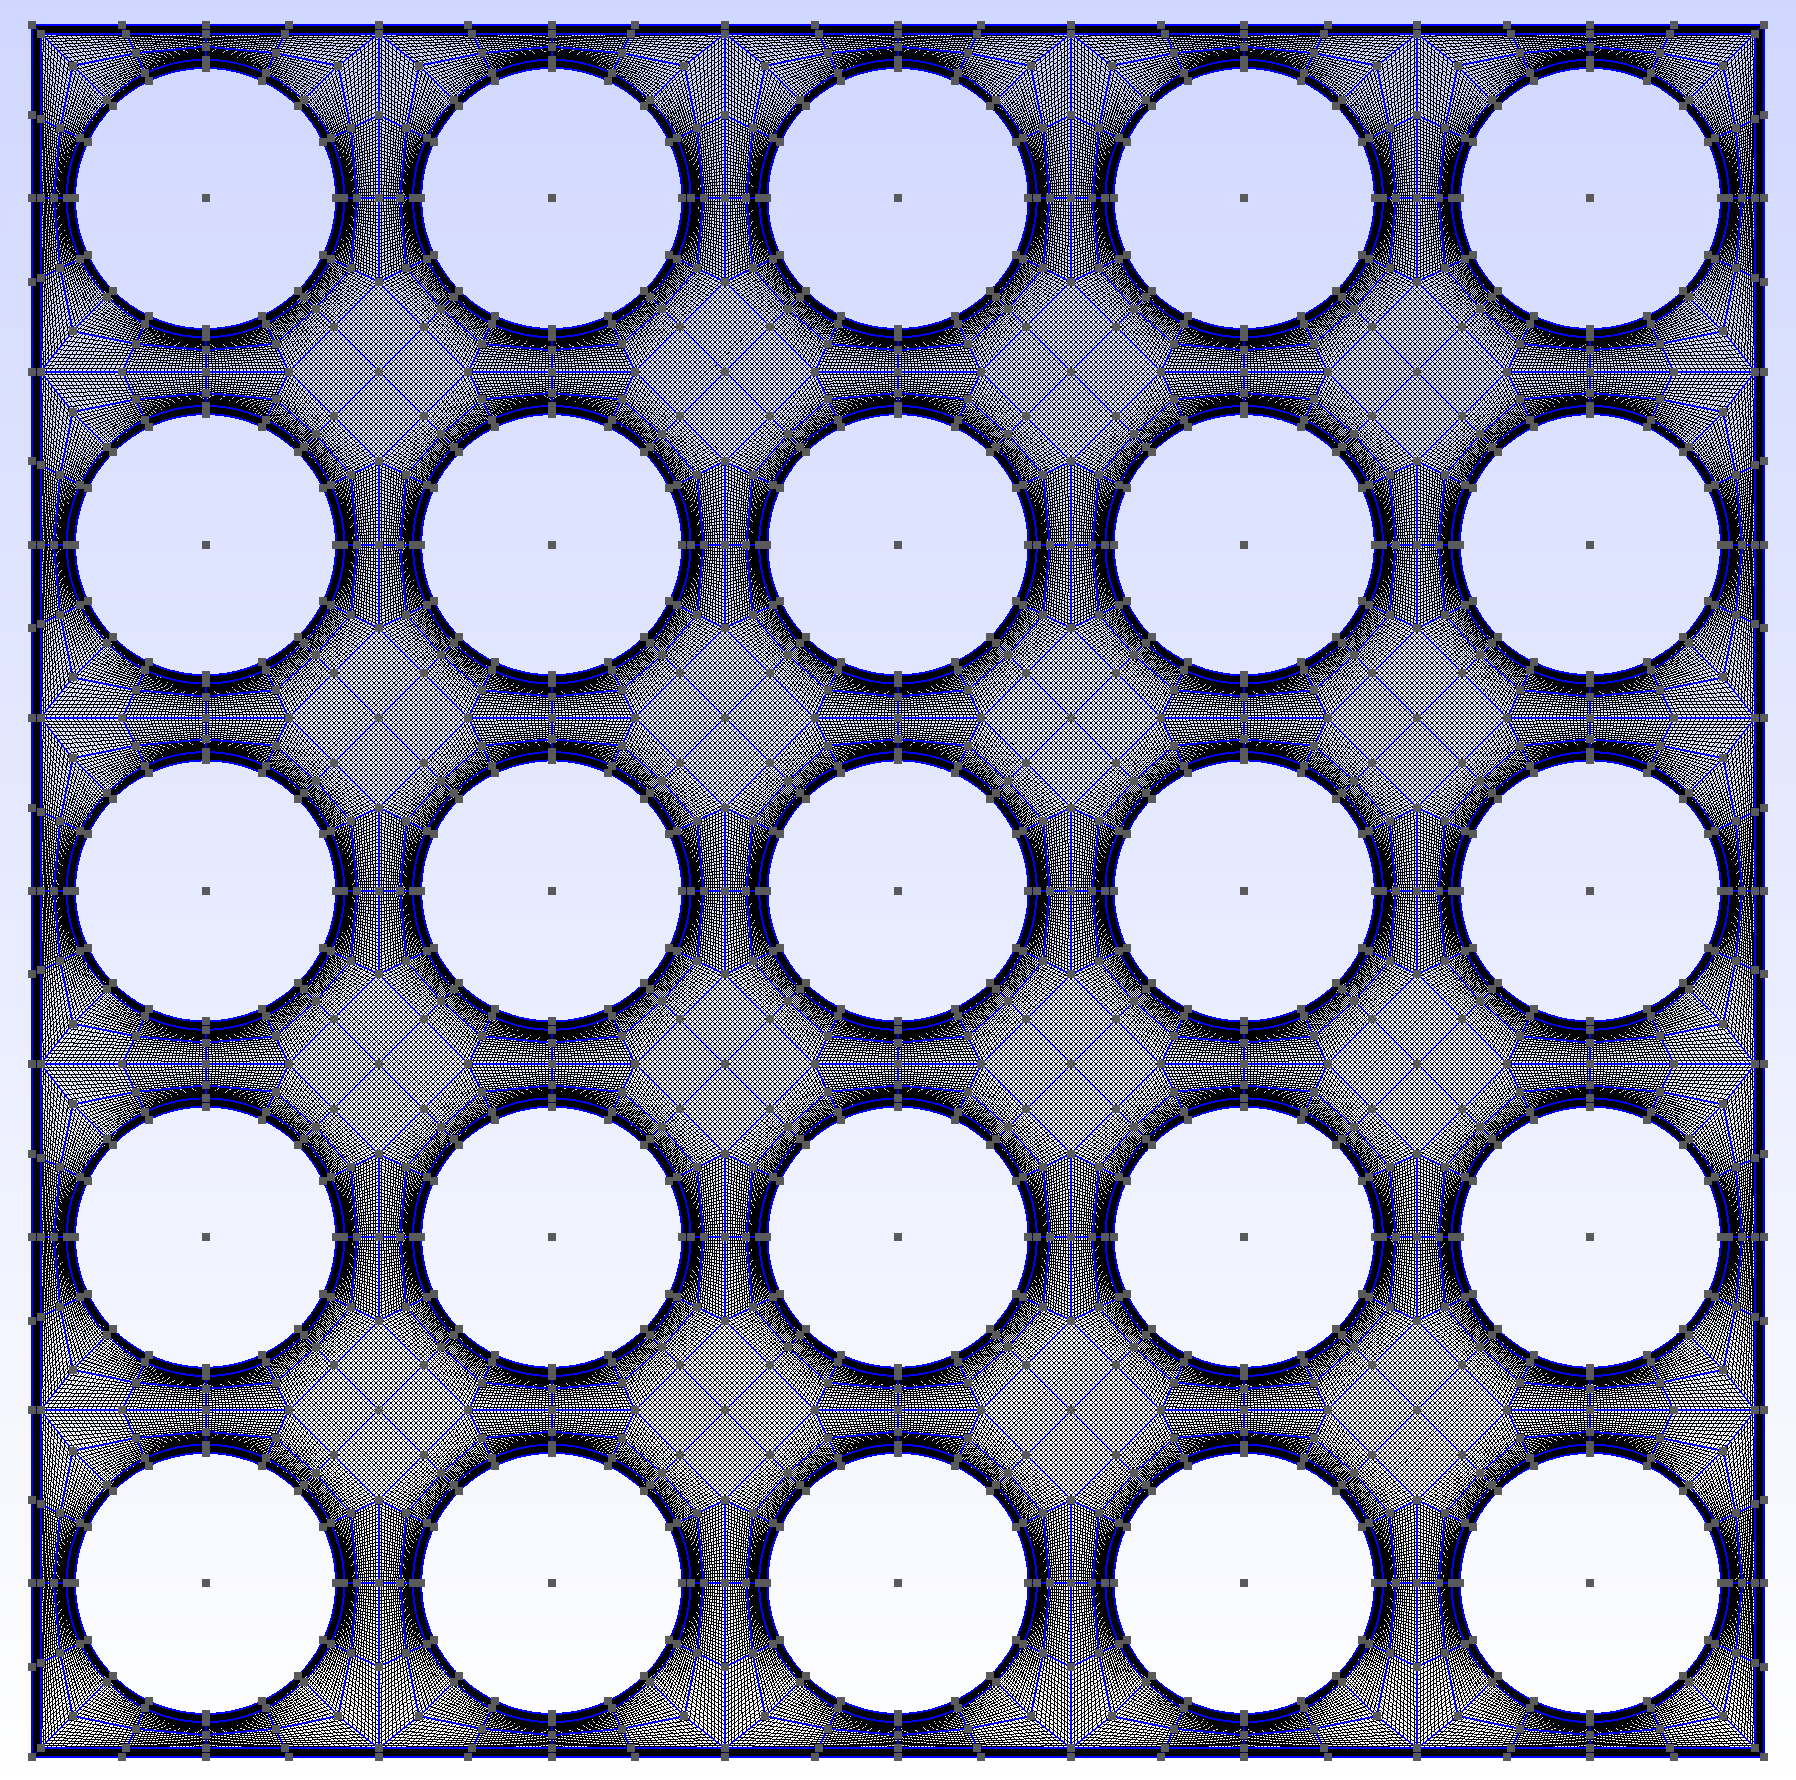
\includegraphics[height = 50mm]{./Figures/ss_thimble/ss_thimble_mesh.png}
%    \caption{.}
%  \end{center}
%\end{figure}


\subsection{Results}

\section{LARGE EDDY SIMULATION}
\label{results_nek5000}

\subsection{Mesh characteristics}



\subsection{Results}

[Some results with Code\_Saturne]

\begin{figure}
\begin{minipage}{0.50\linewidth}
  \begin{center}
    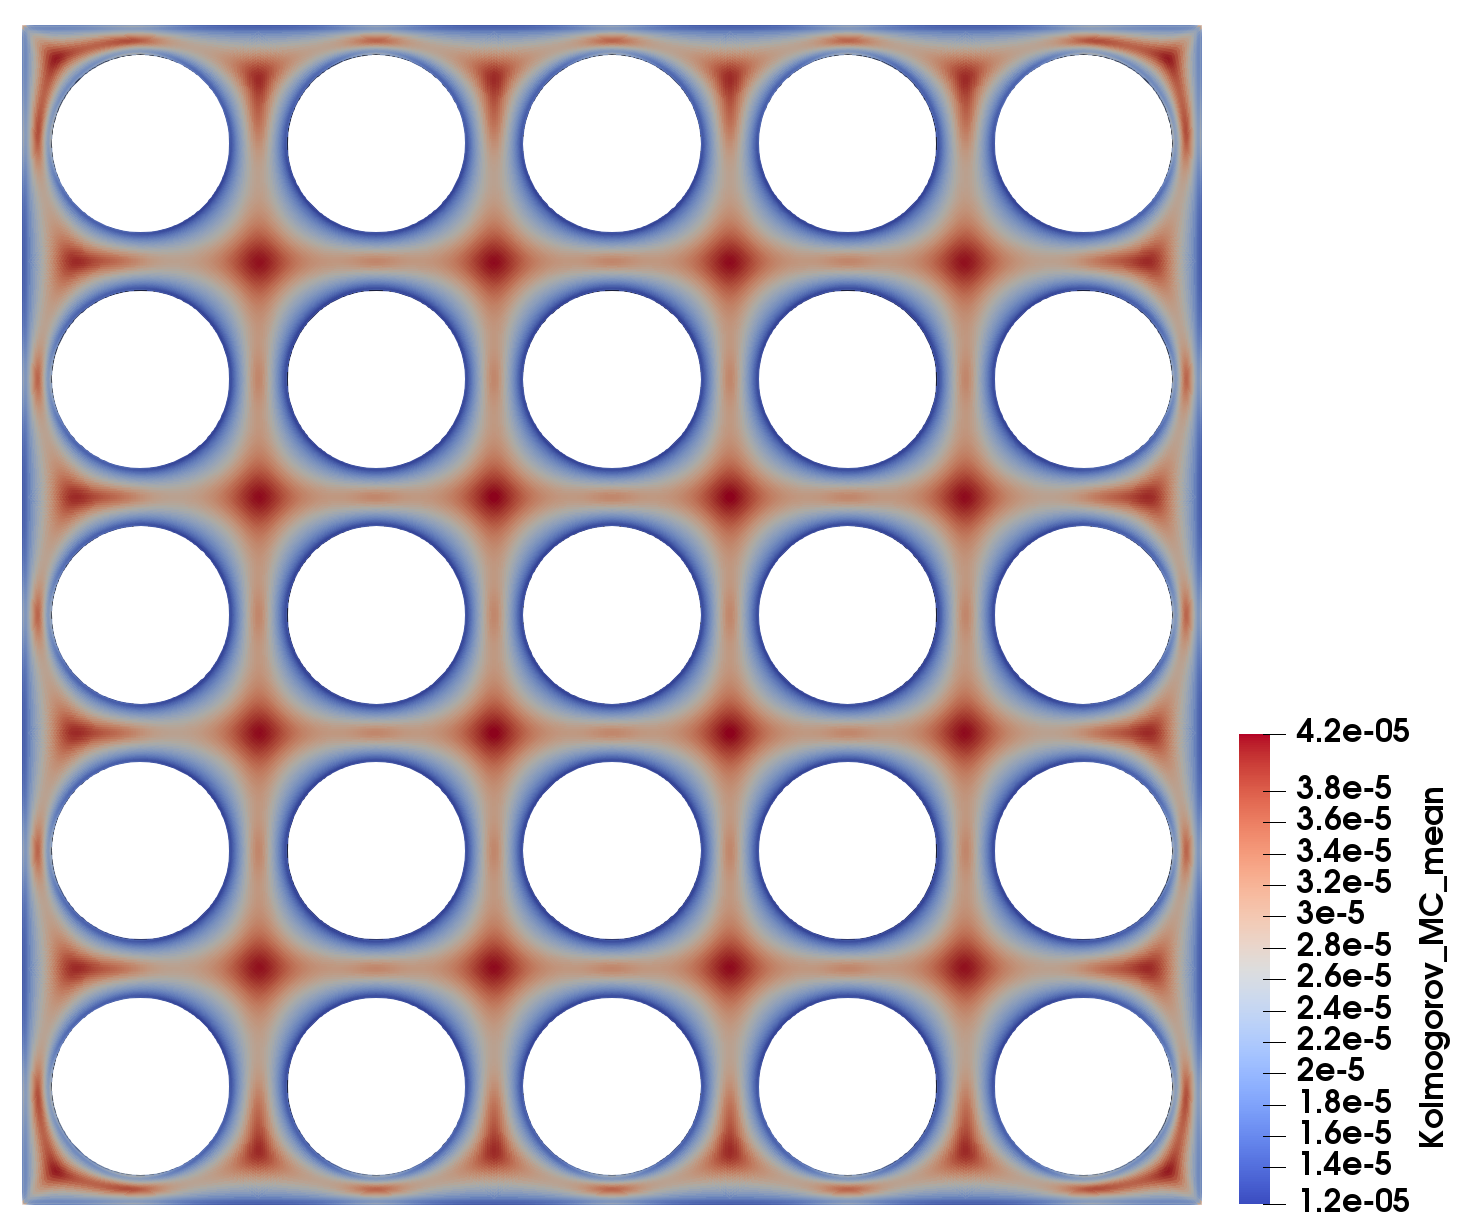
\includegraphics[height = 50mm]{./Figures/ss_thimble/cs_ss_thimble_kolmogorov_mean.png}
    \caption{Kolmogorov length scale (left) and Taylor microscale (right).}
  \end{center}
\end{minipage}\hfill
\begin{minipage}{0.50\linewidth}
   \begin{center}
    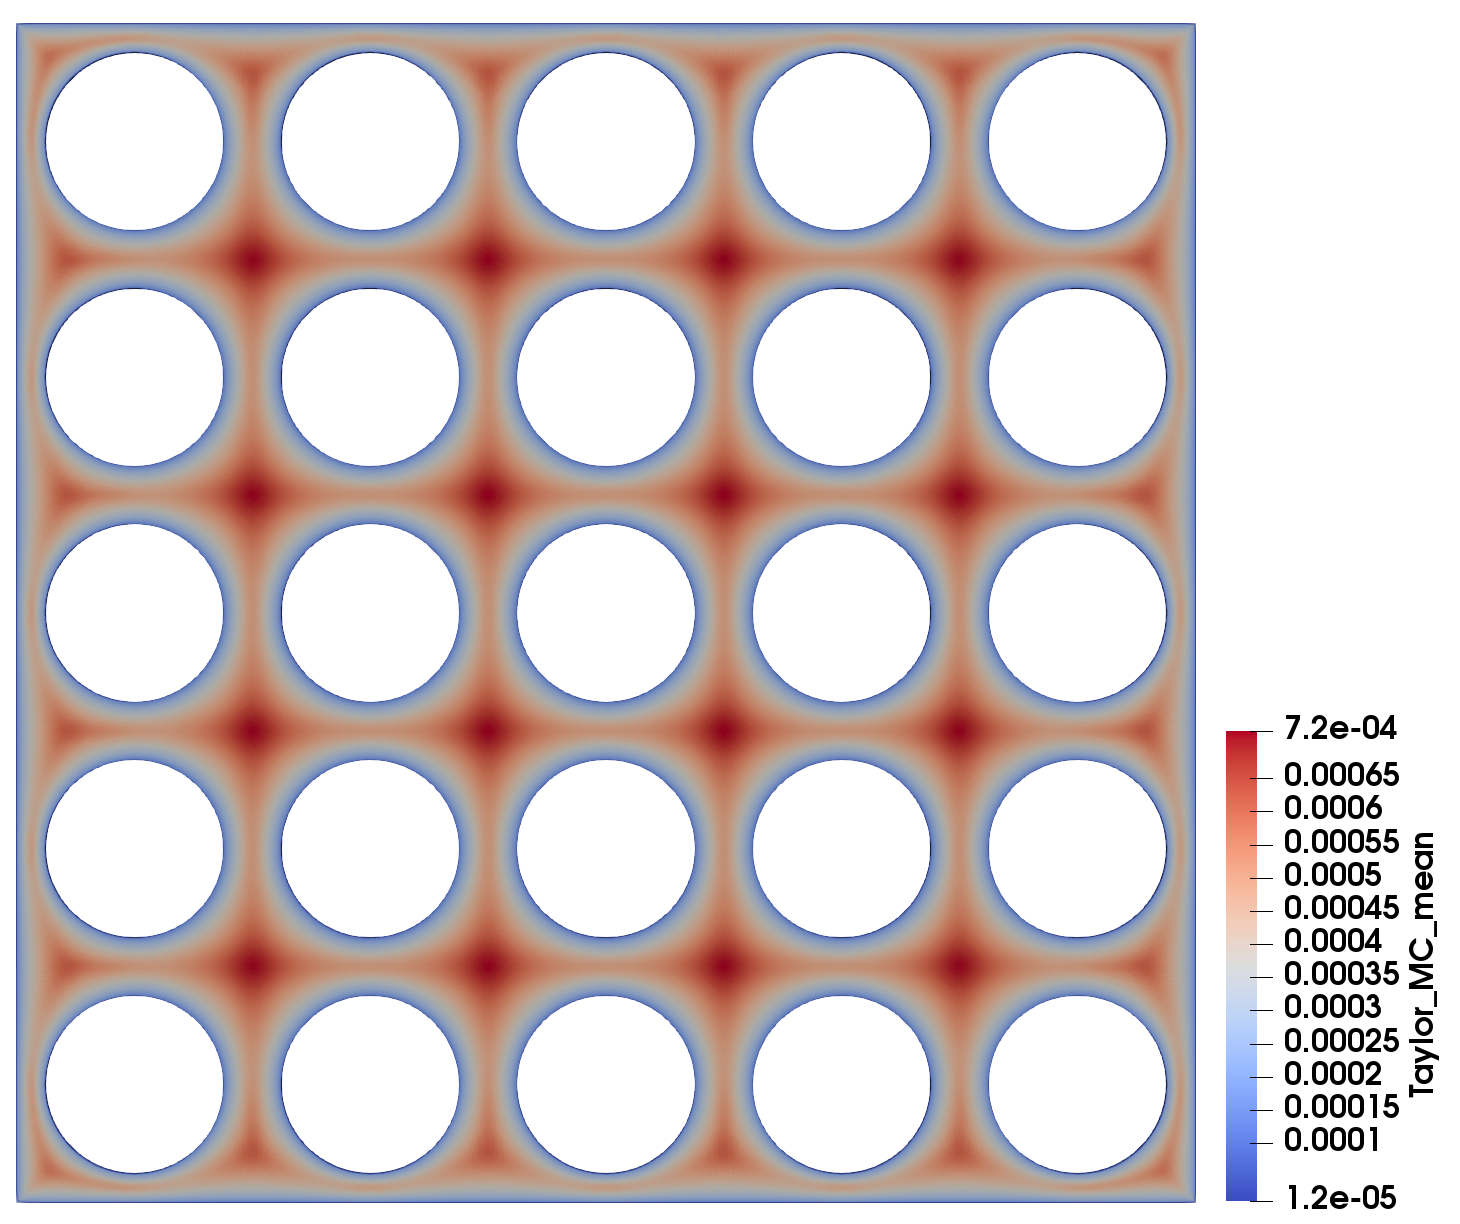
\includegraphics[height = 50mm]{./Figures/ss_thimble/ss_thimble_taylor_mean.png}
    %\caption{Taylor microscale}
   \end{center}
\end{minipage}
\end{figure}



\begin{figure}
\begin{minipage}{0.5\linewidth}
  \begin{center}
    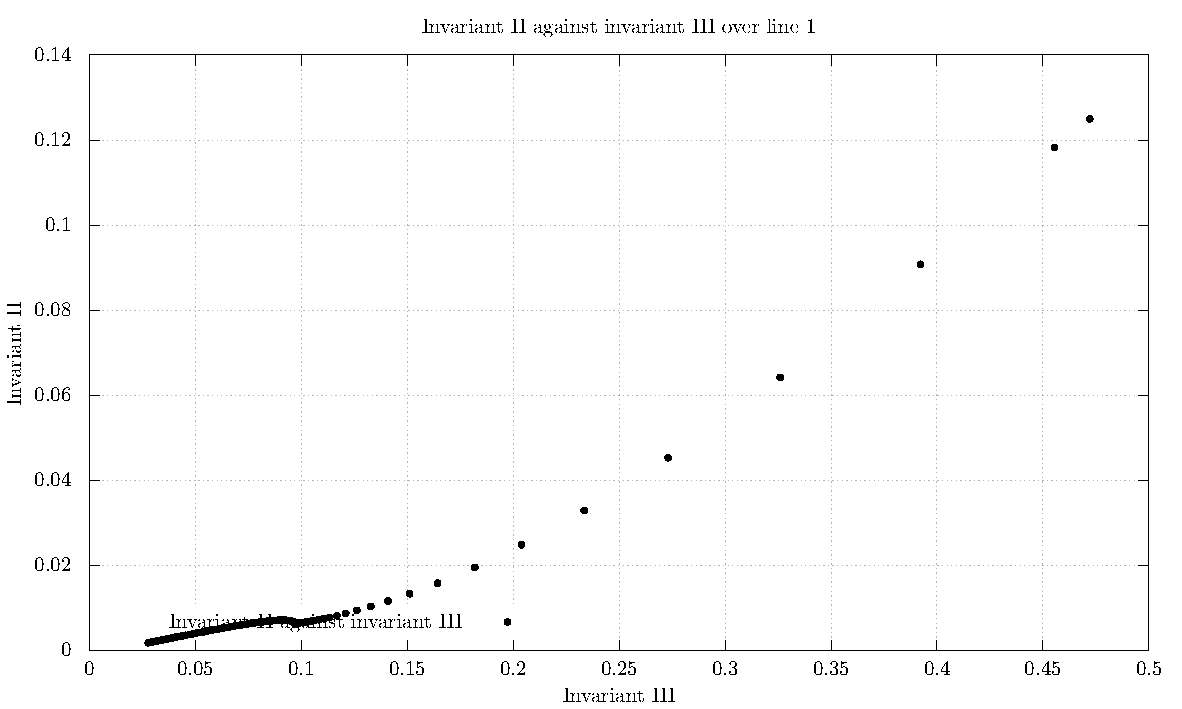
\includegraphics[height = 40mm]{./Figures/cs_lumley1.pdf}
    %\caption{Kolmogorov length scale (left) and Taylor microscale (right).}
  \end{center}
\end{minipage}\hfill
\begin{minipage}{0.5\linewidth}
   \begin{center}
    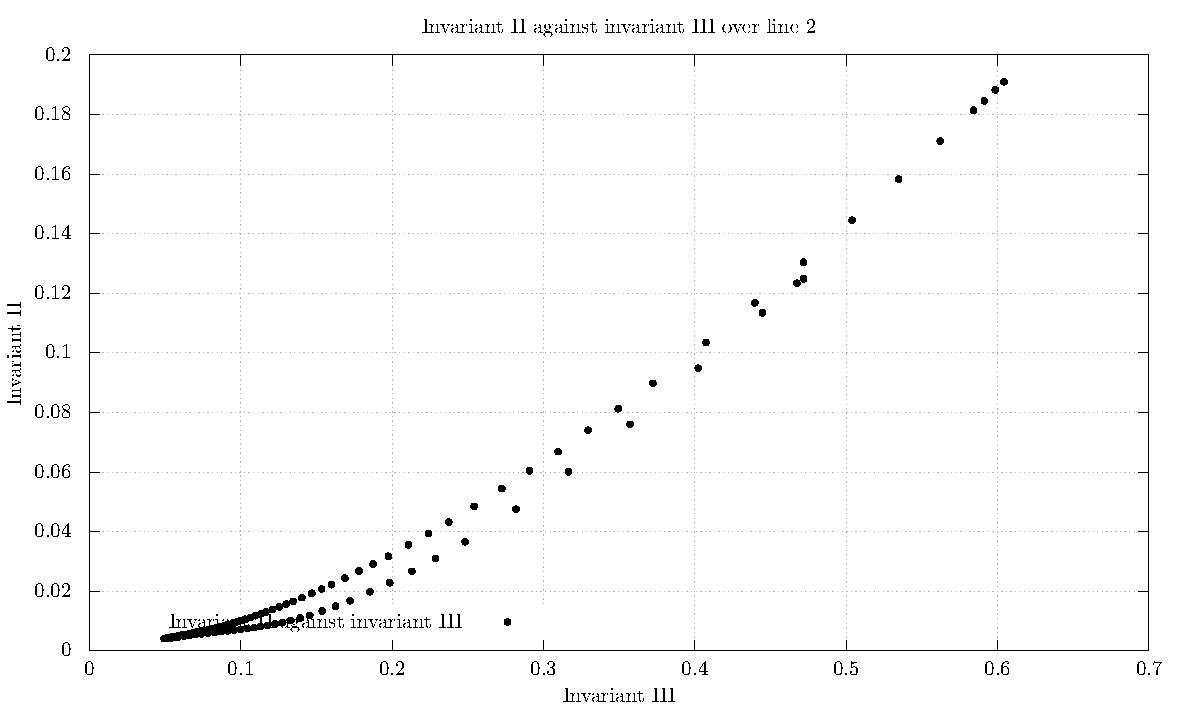
\includegraphics[height = 40mm]{./Figures/cs_lumley2.pdf}
   \end{center}
\end{minipage}
\end{figure}

\begin{figure}
\begin{minipage}{0.5\linewidth}
  \begin{center}
    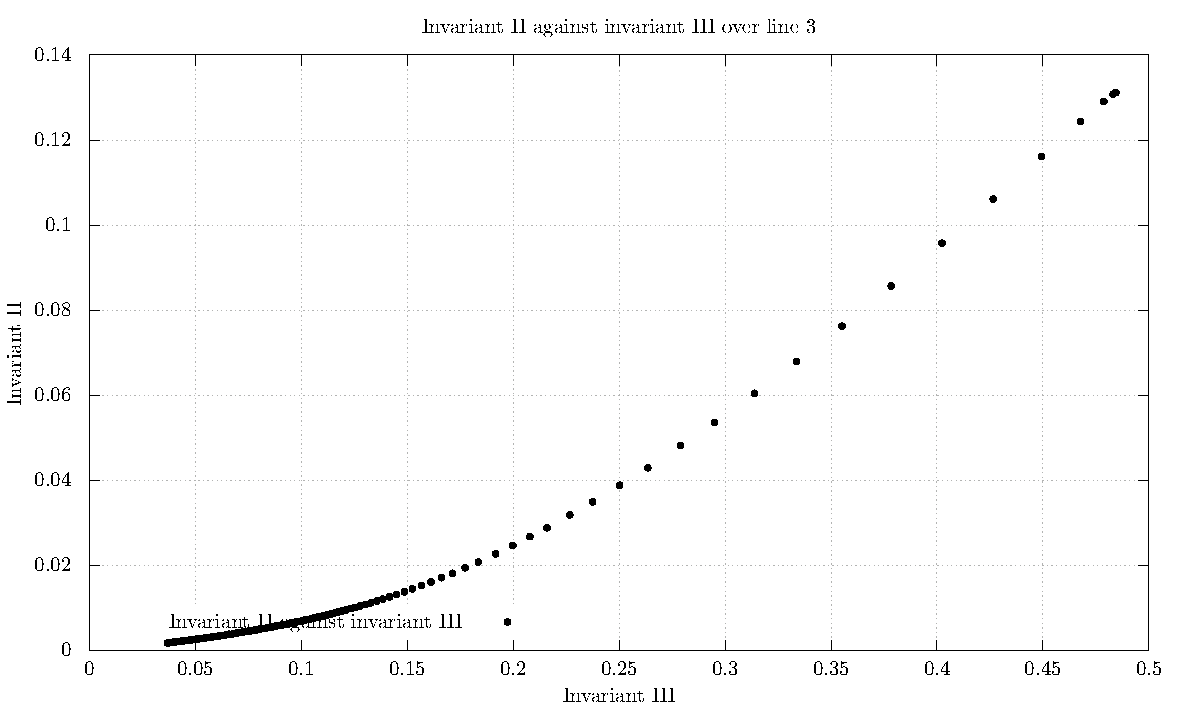
\includegraphics[height = 40mm]{./Figures/cs_lumley3.pdf}
    %\caption{Kolmogorov length scale (left) and Taylor microscale (right).}
  \end{center}
\end{minipage}\hfill
\begin{minipage}{0.5\linewidth}
   \begin{center}
    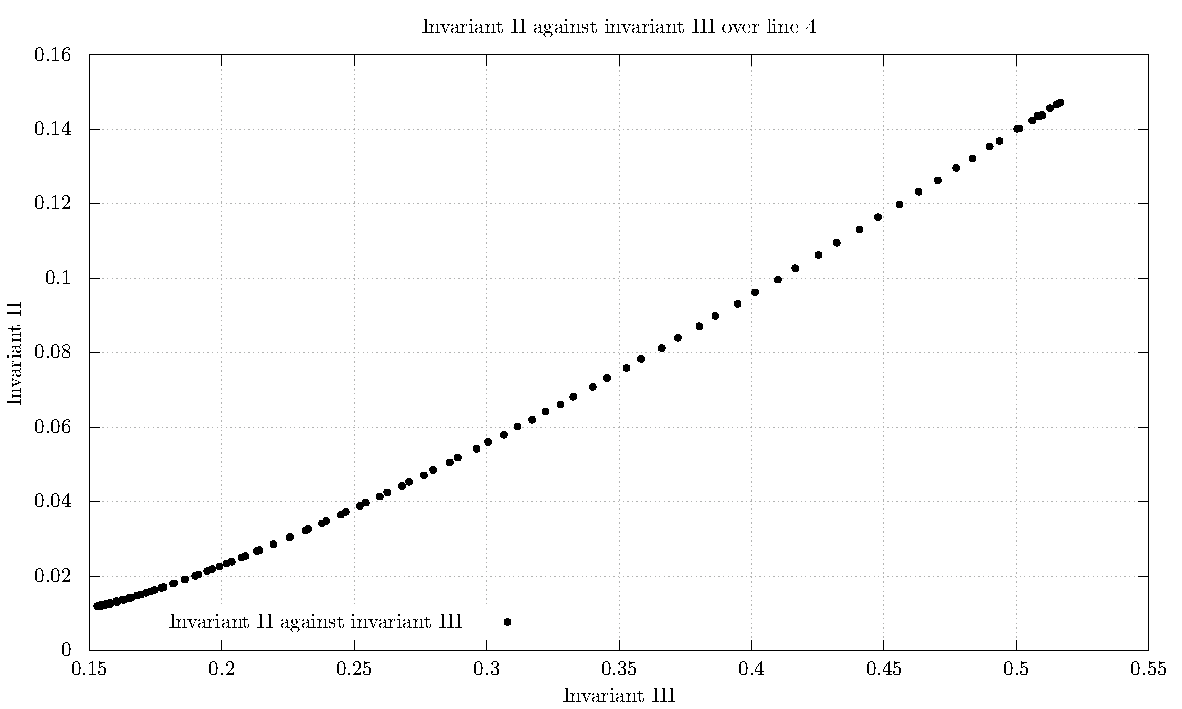
\includegraphics[height = 40mm]{./Figures/cs_lumley4.pdf}
   \end{center}
\end{minipage}
\end{figure}

\begin{figure}
\begin{minipage}{0.5\linewidth}
  \begin{center}
    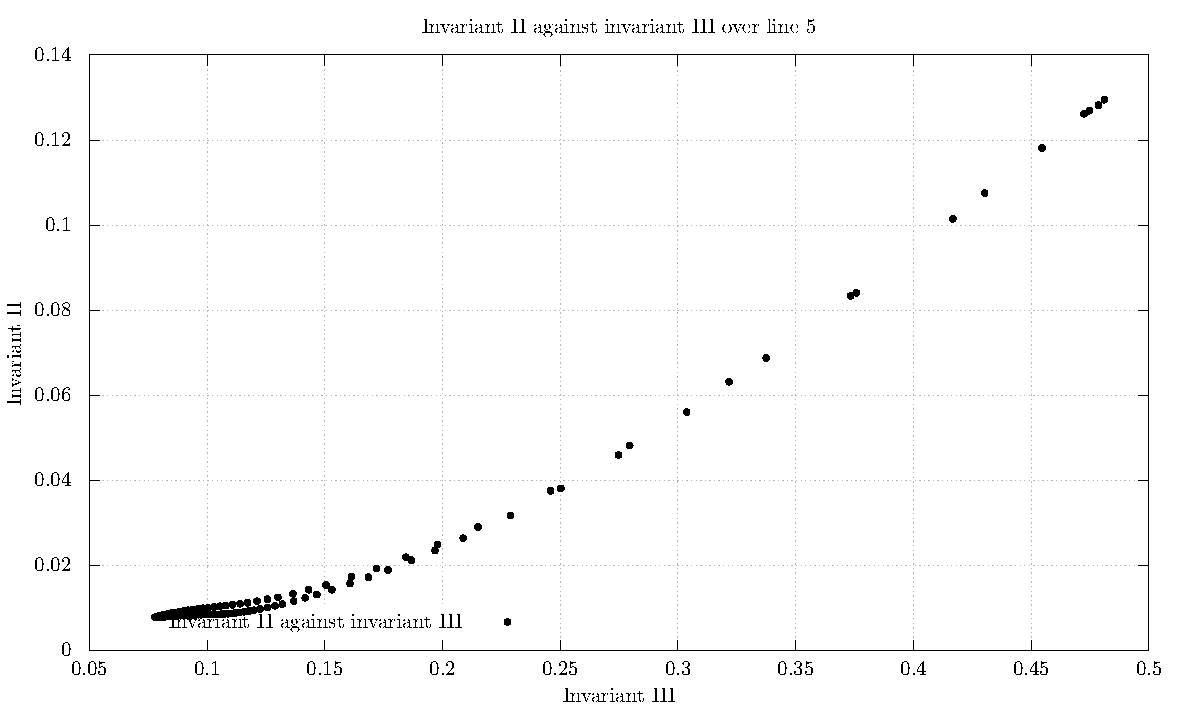
\includegraphics[height = 40mm]{./Figures/cs_lumley5.pdf}
    %\caption{Kolmogorov length scale (left) and Taylor microscale (right).}
  \end{center}
\end{minipage}\hfill
\begin{minipage}{0.5\linewidth}
\end{minipage}
\end{figure}





\section{DISCUSSION}
\label{discussion}

\section{CONCLUSIONS}

%\bibliographystyle{ieeetr}
\bibliographystyle{nureth18new}
%\bibliographystyle{ans}
%\bibliographystyle{plainnat}
%\bibliographystyle{abbrv}
\bibliography{references}

\begin{center}
\scriptsize
\framebox{\parbox{2.6in}{The submitted manuscript has been created by UChicago Argonne, LLC, Operator of Argonne National Laboratory
("Argonne").  Argonne, a U.S. Department of Energy Office of Science laboratory, is operated under Contract No. DE-AC02-06CH11357.  The U.S. Government retains for itself, and others acting on its behalf, a paid-up, nonexclusive, irrevocable worldwide license in said article to reproduce, prepare derivative works, distribute copies to the public, and perform publicly and display publicly, by or on behalf of the Government.}}
\normalsize
\end{center}


\end{document}
